\documentclass[10pt,a4paper]{article}
\usepackage[latin1]{inputenc}
\usepackage{amsmath}
\usepackage{amsfonts}
\usepackage{amssymb}
\usepackage{tikz}
\author{Wendy Moniuk - 996659343}
\title{CSC263 A2}

\usetikzlibrary{arrows}

\tikzset{
 treenode/.style = {align=center, inner sep=0pt, text centered,
    font=\sffamily},
  arn_n/.style = {treenode, circle, black, font=\sffamily\bfseries, draw=black,
    fill=white, text width=1.5em},% arbre rouge noir, noeud noir
  arn_x/.style = {treenode, rectangle, draw=black,
    minimum width=0.5em, minimum height=0.5em}% arbre rouge noir, nil
}

\begin{document}
\begin{enumerate}
\item
\begin{enumerate}

\item
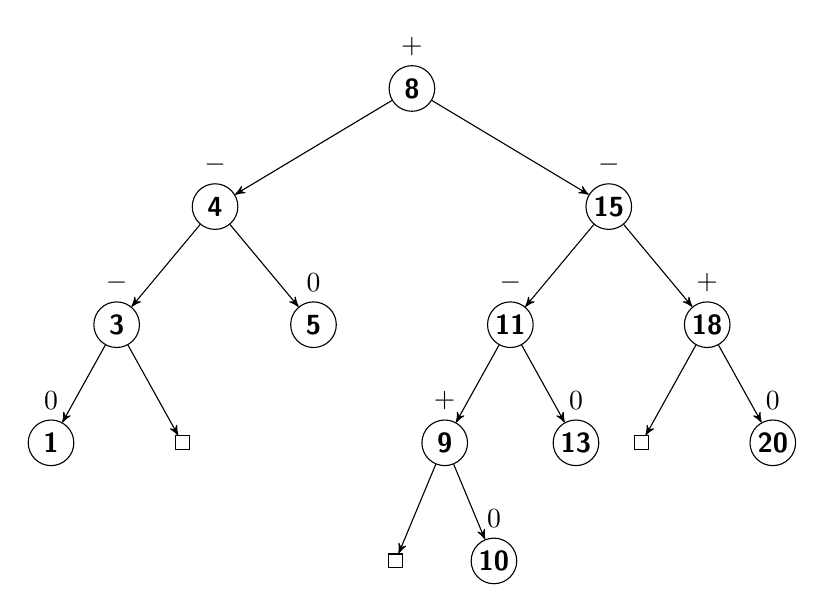
\begin{tikzpicture}[->,>=stealth',level/.style={sibling distance = 5cm/#1,
  level distance = 1.5cm}] 
  \node [arn_n][label=$+$] {8}
  		child{ node [label=$-$][arn_n] {4}
  			child{ node [label=$-$][arn_n] {3}
  				child { node [label=$0$] [arn_n] {1} }
  				child { node [arn_x] {} }
  			}
  			child{ node [label=$0$] [arn_n] {5}
  			}
  		  		}
  		child{ node [label=$-$][arn_n] {15}
  			child{node [label=$-$][arn_n]{11}
  				child{node [label=$+$][arn_n]{9}
  					child{node[arn_x]{}}
  					child{node [label=$0$][arn_n]{10}}
  				}
  				child{node [label=$0$][arn_n]{13}}  			
  			}
  			child{node [label=$+$][arn_n]{18}
  				child{node[arn_x]{}}
  				child{node [label=$0$][arn_n]{20}
  			}  		
  		}
  		};
\end{tikzpicture}

\item
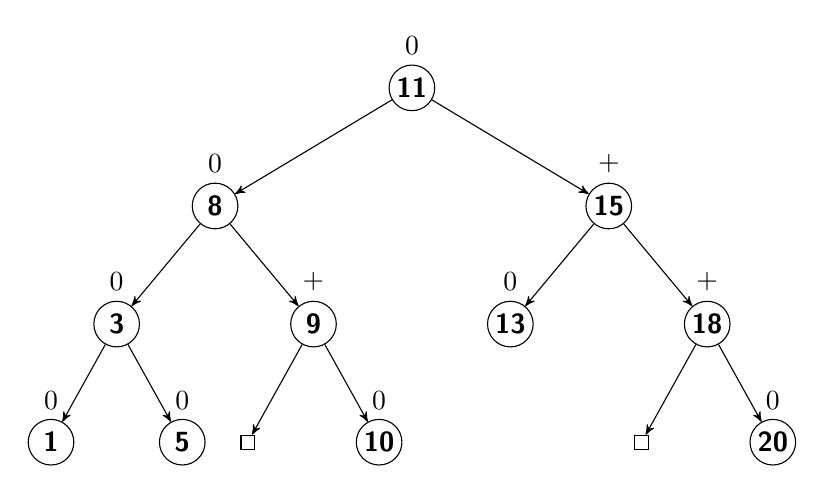
\begin{tikzpicture}[->,>=stealth',level/.style={sibling distance = 5cm/#1,
  level distance = 1.5cm}] 
  \node [arn_n] [label=$0$] {11}
  		child{ node  [label=$0$][arn_n] {8}
  			child{ node [label=$0$] [arn_n] {3}
  				child { node[label=$0$] [arn_n] {1} }
  				child { node [label=$0$][arn_n] {5} }
  			}
  			child{ node[label=$+$] [arn_n] {9}
  				child{ node[arn_x]{}}
  				child{ node [label=$0$][arn_n]{10}}
  			}
  		  		}
  		child{ node[label=$+$] [arn_n] {15}
  			child{node [label=$0$][arn_n]{13}}
  			child{node [label=$+$][arn_n]{18}
  				child{node[arn_x]{}}
  				child{node[label=$0$][arn_n]{20}
  				}  		
  		}
  		}
  		;
\end{tikzpicture}
\end{enumerate}
\item
\begin{enumerate}
\item $m_h = F_{h+1} - F_{h+6}$ with

$F_{-6} = F_{-5} = F_{-4} = F_{-3} = F_{-2} = F_{-1} = F_0 = 0, F_1 = 1; F_h = F_{h-1} + F_{h-2}$

\item
$m_0 = 1 > 1.4^0 - 1 = 0$

$m_1 = 2 > 1.4^1 - 1 = 1$

$m_2 = 3 > 1.96 - 1$

$m_3 = 5 > 2.744 - 1$

$m_4 = 8 > 3.8416 - 1$

Assume that it is true for some $m_h$

Then $m_{h+1} = F_{h+2} - F_{h+7} = F_{h+1} + F_h -(F_{h+6} + F_{h+5})$

$= F_{h+1} - F_{h+6} + F_h - F_{h+5} = m_h + m_{h-1} \geq 1.4^h - 1 + 1.4^{h-1} -1$

$= 1.4^{h-1}(1.4 + 1) -2 = 1.4^{h-1}(2.4) - 2 \geq 1.4^{h+1} - 1$

$1.4^2 = 1.96 \rightarrow$
 if $h > 4$
 then $1.4^{h-1}(1.96+0.44)>1.4^{h+1} + (0.44)1.4^{h-1}> 1.4^{h+1} + 1$
\end{enumerate}
\end{enumerate}
\end{document}
